%
% IMPORTANT: THIS TEMPLATE NEEDS TO BE COMPILED WITH XeLaTeX
%
% This template uses several fonts not included with Windows/Linux by
% default. If you get compilation errors saying a font is missing, find the line
% on which the font is used and either change it to a font included with your
% operating system or comment the line out to use the default font.
%


\documentclass[letterpaper, article]{deedy-resume-openfont}


\begin{document}

%%%%%%%%%%%%%%%%%%%%%%%%%%%%%%%%%%%%%%
%
%     TITLE NAME
%
%%%%%%%%%%%%%%%%%%%%%%%%%%%%%%%%%%%%%%


\namesection{Aaron}{Wubshet}
{ 404.563.9110 | awubshet@mit.edu | www.github.com/aaronwubshet | www.linkedin.com/in/aaronwubshet}

%%%%%%%%%%%%%%%%%%%%%%%%%%%%%%%%%%%%%%
%
%     COLUMN ONE
%
%%%%%%%%%%%%%%%%%%%%%%%%%%%%%%%%%%%%%%
\hfill

\begin{minipage}[t]{0.66\textwidth}
%%%%%%%%%%%%%%%%%%%%%%%%%%%%%%%%%%%%%%
%     EXPERIENCE
%%%%%%%%%%%%%%%%%%%%%%%%%%%%%%%%%%%%%%
\vspace{.01cm}
\section{Experience}
%
% \runsubsection{Bain \& Company}
% \descript{| Associate Consultant Intern}
% \location{Jun - Aug 2018 | Atlanta, GA}
% \vspace{\topsep} % Hacky fix for awkward extra vertical space
% \begin{tightemize}
% 	\item Crash course into management and strategy consulting with seminars on Bain
% 	\item Worked alongside a Bain case team to help a client develop their corporate venture capital business unit
% \end{tightemize}
% \sectionsep
%
% \runsubsection{MIT-HK Innovation Node}
% \descript{| Entrepreneurial \& Maker Intern}
% \location{Jan 2018 | Kowloon Tong, Hong Kong}
% \begin{tightemize}
% 	\item Created a local GSM network test bed via GNU Radio and universal software radio peripherals (USRP)
% 	\item Developed a sector level LTE simulator implemented using MatLab
% \end{tightemize}
% \sectionsep

\runsubsection{Draper}
\descript{| Signal Engineering Intern }
\location{Jan 2017 \& June - Aug 2017 | Cambridge, MA}
\vspace{\topsep} % Hacky fix for awkward extra vertical space
\begin{tightemize}
	\item Created a local GSM network test bed via GNU Radio and universal software radio peripherals (USRP)
	\item Developed a sector level LTE simulator implemented using MatLab to model aggregate power levels
\end{tightemize}
\sectionsep

\runsubsection{Bain \& Company}
\descript{| Building Entrepreneurial Leaders Intern}
\location{Aug 2017 | Atlanta, GA}
\begin{tightemize}
	\item Intro to management and strategy consulting with seminars on Bain workflow
	\item Worked alongside a Bain case team to help a client develop their corporate venture capital business unit
\end{tightemize}
\sectionsep

\runsubsection{MIT Consulting Group}
\descript{| CFO \& Lead Consultant}
\location{Feb 2016 – Present | Cambridge, MA}
\begin{tightemize}
	\item Managed a yearly budget of approximately \$ 50,000 as treasurer while providing clients with a wide array of consulting services
	% including prototype testing, market penetration strategies, employee retention plans, wage matrix evaluation, geographic market analysis, and partnership evaluation.
	\item Clients range from big tech to start-ups to government agencies
\end{tightemize}
\sectionsep

%\runsubsection{MIT Teaching Faculty}
%\descript{| Electrical Engineering and Physics }
%\location{Feb 2016 – Present | Cambridge, MA}
%\begin{tightemize}
%	\item Taught Electricity and Magnetism under Prof. Dourmashkin for 8.02 using the Technology Enabled Active Learning (TEAL) format
%	\item Served as a lab assistant for Theory and Application of Circuits and Electronics on under Prof. Berggren for 6.169
%\end{tightemize}
%\sectionsep

\runsubsection{MIT MakerLodge}
\descript{| Electronics Team Lead and PR Chair}
\location{Feb 2017 – Present | Cambridge, MA}
\begin{tightemize}
	\item Served as the co-head of the electronics training team guiding students through basic a training involving soldering, circuit design, and debugging
	\item Also fulfilled the role of PR Chair to manage interactions with the MIT community and plan social events for mentors
\end{tightemize}

%%%%%%%%%%%%%%%%%%%%%%%%%%%%%%%%%%%%%%%
%%     Projects
%%%%%%%%%%%%%%%%%%%%%%%%%%%%%%%%%%%%%%%

\section{Projects}
\runsubsection{A Drone's Eye View}
\\
\location{Sept - Dec 2017 | Cambridge, MA}
\begin{tightemize}
	\item Drone mounted projector system to turn any surface into an interactive experience with leap motion gesture recognition
	\item Incorporated OptiTrack IR Tracking system, microcomputer programming, and leap motion gesture recognition to create mobile interface system
\end{tightemize}

\runsubsection{Photodiode Amplification}
\\
\location{May - Sept 2017 | Cambridge, MA}
\begin{tightemize}
	\item Designed circuitry and helped structure control software for nanosatellite in Prof. Kerri Cahoy's STAR Lab
	\item Worked with Eagle, LTSpice, Python, and C++ for implementation
\end{tightemize}

\runsubsection{Speaker Tracking System}
\\
\location{Apr - May 2017 | Cambridge, MA}
\begin{tightemize}
	\item Created a target following speaker system that turned to face the target as it moved around as well automatically adjusting the volume
	\item Designed and implemented the system using the Intel 8051 microcontroller as well as Cypress PSoC
\end{tightemize}

\runsubsection{Audio Noise Cancellation}
\\
\location{Mar - Apr 2017 | Cambridge, MA}
\begin{tightemize}
	\item Designed a feedback based noise cancellation system with custom enclosure
	\item Built circuitry to recreate the simulation results on the physical speaker
\end{tightemize}

%\runsubsection{Movie Rating WebApp}
%\\
%\location{September 2016 | Cambridge, MA}
%\begin{tightemize}
%	\item Created a Firebase powered social multimedia platform with a feedback based value system where group members have a time changed vote weight depending on past reliability in picking enjoyable movies
%\end{tightemize}

%\runsubsection{Wireless Charger}
%\\
%\location{Aug 2013 – May 2014 | Lawerenceville, GA}
%\begin{tightemize}
%	\item Designed and built circuitry to wirelessly charge a cell phone from a distance of about one meter as part of an Intel Science Fair project submission
%\end{tightemize}
%\sectionsep

%%%%%%%%%%%%%%%%%%%%%%%%%%%%%%%%%%%%%%
%     RESEARCH
%%%%%%%%%%%%%%%%%%%%%%%%%%%%%%%%%%%%%%

%\section{Research}
%
%\runsubsection{RLE at MIT}
%\descript{| Research Assistant}
%\location{Nov 2015 – May 2016 | Cambridge, MA}
%\begin{tightemize}
%	\item Experimentalist and data analyst under Marin Sojacic creating transparent displays with silver and gold nanoparticles dispersed in a polymer matrix
%	\item Experimented with possible ratios of specific nanoparticles to polymer while accounting for size and identity in order to sharpen resonant scattering\\
%\end{tightemize}
%\sectionsep
%
%\runsubsection{Quantum Chemistry Lab at GT}
%\descript{| Research Assistant}
%\location{Aug 2014 – May 2015 | Atlanta, GA}
%\begin{tightemize}
%	\item Experimental apparatus designer under Ken Brown constructing additional laser modulation systems via direct digital synthesis
%	\item Worked with Ca\textsuperscript{2+} ion trapping to investigate quantum states and computers
%\end{tightemize}


\end{minipage}
\hfill
%%%%%%%%%%%%%%%%%%%%%%%%%%%%%%%%%%%%%%
%
%     COLUMN TWO
%
%%%%%%%%%%%%%%%%%%%%%%%%%%%%%%%%%%%%%%
\begin{minipage}[t]{0.33\textwidth}

%%%%%%%%%%%%%%%%%%%%%%%%%%%%%%%%%%%%%%
%     EDUCATION
%%%%%%%%%%%%%%%%%%%%%%%%%%%%%%%%%%%%%%
\vspace{\topsep}
\centering{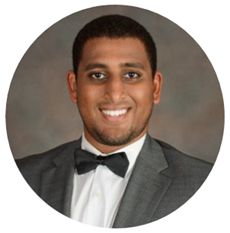
\includegraphics{resume_image.png}}


\section{Education}

\subsection{Massachusetts Institute of Technology \hfill}
\descript{{\large BS in Electrical Engineering}}
\location{June 2019 | Cambridge, MA \\ GPA: 4.4}
\sectionsep

\subsection{Relevant Coursework \hfill}
\vspace{.05cm}
6.302: Feedback Systems and Controls\\
6.115: Microcomputer Project Laboratory \\
6.111: Digital Systems Laboratory \\
6.S063: Engineering Interactive Technologies



%%%%%%%%%%%%%%%%%%%%%%%%%%%%%%%%%%%%%
%     SKILLS
%%%%%%%%%%%%%%%%%%%%%%%%%%%%%%%%%%%%%%

\section{Skills}
\subsection{Technical}

Verilog/BSV \hspace{2.625cm} \textbullet \textbullet  \textbullet \textbullet \textbullet \\
MatLab \hspace{3.28cm} \textbullet \textbullet \textbullet \textbullet  \textbullet\\
Eagle \hspace{3.63cm} \textbullet \textbullet \textbullet \textbullet \\
Mechanical CAD Software \hspace{.5cm} \textbullet \textbullet  \textbullet \\
Python \hspace{3.37cm}  \textbullet \textbullet  \textbullet \\






\sectionsep

\subsection{Management}
Accounting \hspace{2.75cm} \textbullet \textbullet \textbullet  \textbullet \textbullet\\
Logistics \hspace{3.15cm} \textbullet \textbullet  \textbullet \textbullet \\
Resource Allocation \hspace{1.47cm} \textbullet \textbullet \textbullet \textbullet \\
Mentorship \hspace{2.7cm} \textbullet \textbullet \textbullet  \\



\section{Research}

\subsection{Research Laboratory of \hfill}
\subsection{Electronics (RLE) at MIT \hfill}
Experimentalist under Prof. Marin Sojacic creating transparent displays with nanoparticles dispersed in polymer matrix
\sectionsep
\subsection{Cold Molecules and \hfill}
\subsection{Quantum Information \hfill Lab at GT \hfill}
Experimental apparatus designer under Prof. Ken Brown working with laser modulation system to ion trap Ca\textsuperscript{2+}
%\sectionsep
%\subsection{Intel Science Fair \hfill}
%Designed wireless charging apparatus self-testing photodiode amplifier module for nanosat electronics team working under Prof. Kerri Cahoy
%\sectionsep


\end{minipage}

\end{document}
